\documentclass{estilo}
\usepackage[spanish]{babel}
\usepackage{graphicx}
\usepackage{float}
\usepackage{amsmath}        % para los vectores columnas
\usepackage{amsfonts}       % para las negrita de pizarra
\usepackage{amssymb}        % para simbolos matematicos
\usepackage{hyperref}       % para utilizar referencias
\usepackage{multirow}       % para las tablas
\usepackage{dsfont}
\usepackage{listings}
\usepackage{xcolor}
\definecolor{codegreen}{rgb}{0,0.6,0}
\definecolor{codegray}{rgb}{0.5,0.5,0.5}
\definecolor{codepurple}{rgb}{0.58,0,0.82}
\definecolor{backcolour}{rgb}{0.95,0.95,0.92}
\lstdefinestyle{mystyle}{
    backgroundcolor=\color{backcolour},   
    commentstyle=\color{codegreen},
    keywordstyle=\color{magenta},
    numberstyle=\tiny\color{codegray},
    stringstyle=\color{codepurple},
    basicstyle=\ttfamily\footnotesize,
    breakatwhitespace=false,         
    breaklines=true,                 
    captionpos=b,                    
    keepspaces=true,                 
    numbers=left,                    
    numbersep=5pt,                  
    showspaces=false,                
    showstringspaces=false,
    showtabs=false,                  
    tabsize=2
}
\lstset{style=mystyle}

\usepackage{enumitem,multicol,setspace}
\newcounter{subenum}[enumi] % para las multicolumnas
\renewcommand{\thesubenum}{\arabic{subenum}}
\usepackage[nomessages]{fp}
\FPeval\thecolwidth{round(1/4:4)}% Specify number of columns -> column width
\newcommand{\newitem}[1]{%
  \refstepcounter{subenum}%
  \parbox{\dimexpr\thecolwidth\linewidth-.5\columnsep}{%
    \makebox[\labelwidth][r]{(\thesubenum)\hspace*{\labelsep}}%
    #1}\hfill%
}

\usepackage{scalerel,stackengine} % para el sombrero
\stackMath
\newcommand\rhat[1]{%
\savestack{\tmpbox}{\stretchto{%
  \scaleto{%
    \scalerel*[\widthof{\ensuremath{#1}}]{\kern-.6pt\bigwedge\kern-.6pt}%
    {\rule[-\textheight/2]{1ex}{\textheight}}%WIDTH-LIMITED BIG WEDGE
  }{\textheight}% 
}{0.5ex}}%
\stackon[1pt]{#1}{\tmpbox}%
}
\parskip 1ex

\usepackage{mathtools}      % floor y ceil
\DeclarePairedDelimiter\ceil{\lceil}{\rceil}
\DeclarePairedDelimiter\floor{\lfloor}{\rfloor} 

\usepackage[style=authoryear-comp]{biblatex}

\begin{document}
\maketitle

\justifying{}

\newpage
\section{Introducción}

La finalidad del presente trabajo práctico consiste en el planteamiento y análisis de un algoritmo que logre determinar cuál sería la \textit{mejor estrategia} de ataque para la policía secreta de Ba Sing Se, los Dai Li, frente al \textit{ataque ráfaga} que la nación del fuego efectuará. 

Para el plantemiento de dicho algoritmo resulta imprescindible llevar a cabo un análisis exhaustivo del problema mismo: su forma y composición, y finalmente la ecuación de recurrencia del mismo. 

Una vez consolidada nuestra propuesta de algoritmo, expondremos el análisis correspondiente al mismo, considerando factores de nuestro interés como la complejidad temporal y espacial del mismo, así como los efectos de la variabilidad de los valores dados sobre los tiempos de ejecución y sobre la optimalidad de la solución a la que llegamos.\\



\textbf{Sobre la estrategia a obtener:}
{\setlength{\parindent}{25pt}
\begin{itemize}
    \item El criterio para considerar una estrategia como $mejor$ se basa en que la misma \textbf{maximice la cantidad de bajas totales} en las tropas enemigas.
    \item  La estrategia resultante debe indicar en qué minutos resulta más conveniente llevar a cabo un ataque (empleando el total de energía disponibe hasta ese momento) así como cuándo no atacar, es decir, usar ese tiempo para cargar la energía disponible para el próximo ataque.\\
\end{itemize}
}


\textbf{Sobre la información disponible:}
{\setlength{\parindent}{25pt}

\begin{itemize}
    \item El \textit{ataque ráfaga} que la nación del fuego planea llevar a cabo consiste en una susesión de hordas de soldados aproximándose cada minuto, misma que durará $n$ minutos.
    \item Es conocida la cantidad de soldados con los que cuenta cada horda, en cada minuto $i\in\mathbb{N}/ \\ i\leq n$. Esta cantidad la representamos como $x_i$.
    \item También conocemos qué intesidad tiene un ataque de los Dai Li, es decir, cuántas bajas podría generar en las tropas enemigas (ya que de no haber soldados, aún si se tiene una intensidad alta , no se genera ninguna baja) respecto al tiempo de carga de energía. Esta cantidad la representamos como $f_i$
\end{itemize}

}


\justifying{
\section{Análisis del problema}\label{sec:analisisProblema}
En esta sección expondremos la información con la que disponemos y cómo es que ideamos el procedimiento representado en el algoritmo propuesto.

Dados los datos de entrada, denominaremos:
\begin{itemize}
    \item Cantidad de minutos a considerar ($n$).
    \item Cantidad de soldados que llegarán en el i-ésimo minuto ($x_i$).
    \item Capacidad de eliminación de soldados si transcurrieron j minutos desde el anterior ataque ($f_j$, sea $j<=i$).
\end{itemize}

Para encontrar la solución general, buscamos que de la solución de los subproblemas previos obtengamos los siguiente datos de forma iterativa:
\begin{itemize}
    \item Cantidad de eliminaciones maximizadas de atacar en el minuto i/muertes óptimas en el minuto i ($OP(i)$)
    \item Minuto del reinicio de energía previo más reciente ($reinicio_i$).
    \item Energia disponible dado $reinicio_i=k$  ($e_k$).
\end{itemize}

\setlength{\parindent}{0cm}Una consideración que tuvimos en cuenta fue que al maximizar iterativamente las muertes que podriamos provocar con nuestra estrategia, parece conveniente siempre atacar en el último minuto. Esto podría llevar a que si se toma una estrategia óptima de manera fija para la formación de estrategias futuras podriamos estar incurriendo en el error de no reevaluar su optimalidad ante otras estrategias que ya vendriamos habiendo construido y que tendríamos hasta ese punto en disposición. Centraremos el analisis de las soluciones de los subproblemas pasados de forma en que estos me puedan ayudar a construir la solución de subrpoblemas más grandes, concretamente buscaremos definir qué subestratégia óptima previa nos permitirá llegar con la energía necesaria para obetener resultados óptimos para el subrpoblema que se esté analizando. 

\setlength{\parindent}{0cm}Adicionalmente, mencionamos que la energía disponible después del último ataque realizado en el minuto k ($e_k$) no es más que los minutos que transcurrieron a partir del minuto k.

\setlength{\parindent}{0cm}Veamos cómo podemos encarar nuestro problema a través del análisis de breve. Sea $n = 3$:

\begin{center}
\begin{tabular}{ |c|c|c|c| }
\hline
\textbf{$x_i$} & 900 & 600 & 800 \\ \hline
\textbf{$f_i$} & 100 & 150 & 600 \\
\hline
\end{tabular}
\end{center}

\paragraph{En el minuto $i=0$:} No hay rafagas de soladados que matar y no hubo reinicio previo (\textit{No podemos atacar}). Es decir: $OP(0)=0$.

\paragraph{En el minuto $i=1$:} Sabiendo que siempre nos conviene atacar en el último minuto solo tenemos que definir con cuánta energía. Solo tenemos \textbf{una opción} puesto que solo podemos llegar con energía = 1 ($e_0=1)$. Por lo tanto, con  $reincio_1=0$: $OP(1)=100$.


\paragraph{En el minuto $i=2$:} Ahora contemplamos \textbf{2 opciones}: Eliminar o a 150 o a 100 soldados de la horda actual. Para poder eliminar a 150 deberíamos haber llegado a este minuto con energía = 2 (es decir: $reinicio_2=0$) y tendríamos las eliminaciones que ya llevabamos hasta el minuto de reincio (en este caso ninguna pues $OP(0)=0$), mientras que para poder eliminar a 100 soldados necesitaríamos llegar con energía = 1 (es decir: $reinicio_2=1$) contando entonces con las 100 eliminaciones realizadas hasta el minuto de reinicio de la opción considerandose (pues $OP(1)=100$). En otras palabras, las posibles muertes a lo largo de la batalla que podemos generar son:

\begin{itemize}
    \item $reinicio_2=0$: $OP(0)$ + 100 = 0+150 = 150 eliminaciones.
    \item $reinicio_2=1$: $OP(1)$ + 150 = 100+100 = 200 eliminaciones.
\end{itemize}
Podemos entonces concluir que tomando $reinicio_2=1$, nuestro óptimo es $OP_2 = 200$,

\paragraph{En el minuto $i=3$:} Contemplamos \textbf{3 opciones}: Eliminar o a 600, a o a 150 o 100 soldados de la horda actual. Eliminar a 100 implica $reinicio_3=0$ entonces las muertes ya optimizadas que adiciono son $OP(0)=0$; a su vez, eliminar a 150 implica $reinicio_3=1$ entonces las muertes ya optimizadas que adiciono son $OP(1)=100$; finalmente, eliminar a 100 implica $reincio_3=2$ entonces las muertes ya optimizadas que adiciono son $OP(2)=200$. En otras palabras:

\begin{itemize}
    \item Sin previo reinicio $reinicio_3=0$: $OP(0)$ + 600 = 0+600 = 600 eliminaciones.
    \item Previo reinicio en $reinicio_3=1$: $OP(1)$ + 150 = 100+150 = 250 eliminaciones.
    \item Previo reinicio en $reinicio_3=2$: $OP(2)$ + 100 = 200+100 = 300 eliminaciones.
\end{itemize}
Entonces, con $reinicio_3=0$: $OP(3) = 600$. 

\paragraph{Al terminar la batalla:} La máxima cantidad de eliminaciones que logramos producir fue de 600 soldados y los datos obtenidos de las soluciones iterativas fueron:

\begin{center}
\begin{tabular}{ |c|c|c|c|c| }
\hline
\textbf{$OP(i)$} & 0 & 100 & 200 & 600 \\ \hline
\textbf{$reinicio_i$} & 0 & 0 & 1 & 0 \\
\hline
\end{tabular}
\end{center}

Bajo el esquema presentado, podemos realizar la reconstrucción de la estrategía que nos llevó a la cantidad de eliminaciones calculada. En general, dados los reinicios, si retrocedemos desde el final hasta llegar al minuto 0 (donde no hay ataques previos) podremos ubicar los minutos en los que hemos realizado un ataque (por ende un reinicio de energía). En este ejemplo, como $reinicio_3=0$ entonces el primer y último ataque fue en dicho minuto: CARGAR, CARGAR,ATACAR. 

Algunos puntos que nos gustaría extraer del ejemplo desarrollado:
\begin{itemize}
    \item{No siempre maximizar la cantidad de eliminaciones en la rafaga actual implica mejores resultados. Vease el análisis para $i=2$.}
    \item{El tener en cuenta las estrategias óptimas previas nos facilita el no tener que calcular la estrategia previamente usada al último reinicio de energia. Entonces no evaluamos estrategias con un mismo último reinicio de energia que no sean las mejores.}
    \item{Todo óptimo futuro se compone de alguno de los óptimos pasados (incluyendo, y en especial, a  $OP(0)=0$).}
    \item{Para escoger de entre las muertes que podamos generar en un minuto analizamos las opciones previas y maximizamos la suma de las muertes con las que contabamos hasta el reinicio que la opción que estoy evaluando implica y las muertes que genero en ese minuto.}


\end{itemize}


\subsection{Forma y composición del problema} Analizaremos cómo se comporta nuestro problema respecto a 2 ámbitos generales: la forma de los subproblemas y el cómo estos se componen para solucionar subproblemas más grandes. Es decir, evaluaremos someramente cómo se complica el problema al aumentar los minutos que durará el ataque de la nación del fuego ($n$). Más adelante, en el análisis de los efectos de la variablidad de datos podremos contemplar la concretización de las proposiciones planteadas.\\

En principio, estipulamos que en el minuto 0, cuando no hay ninguna rafaga de soldados con los que tengamos que lidiar, la solución obvia es el no atacar (no tenemos ni energias ni objetivos que eliminar). Adicionalmente, si el tiempo total de duración de la batalla es $n$, no hay situación en la que no nos convenga atacar en este preciso minuto.Además, decimos que la complejidad de nuestro problema se encuentra en evaluar los soldados que podríamos eliminar con cierta energía teniendo en cuenta el óptimo que se tendría que tomar para poder eliminar los propuestos para esa horda. A continuación, estudiaremos el cómo se complica nuestro problema basandonos en la cantidad de opciones entre las que debemos encontrar la que nos funciona mejor para lograr la optimalidad.

\subparagraph{¿Cómo se complica nuestro problema al incrementar $n$?} 
\begin{itemize}
    \item Cuando $n=1$ la \textbf{única opción} de energia es 1 (no hubo oportunidad de atacar)
        \begin{center}
        \begin{tabular}{ |c|c|c| }
        \hline
         \textbf{Opción 1:} sin reinicio & estrategia óptima hasta minuto 0& \textit{atacar} \\
         \hline
        \end{tabular}
        \end{center}
        
    \item Cuando $n=2$ puedo llegar con \textbf{2 opciones de energia}: 1 o 2. Mis alternativas de estrategia son: 
        \begin{center}
        \begin{tabular}{ |c|c|c| }
        \hline
         \textbf{Opción 1:} sin reinicio& estrategia óptima hasta minuto 0& \textit{atacar} \\
         \hline
         \textbf{Opción 2:} reinicio en 1& estrategia óptima hasta minuto 1& \textit{atacar} \\
        \hline
        \end{tabular}
        \end{center}
        
    \item Cuando $n=3$ puedo llegar con \textbf{3 opciones de energia}: 1, 2 o 3 (llegar con energia k implica usar la estrategia óptima para llegar con esa energia).
        \begin{center}
        \begin{tabular}{ |c|c|c|c| }
        \hline
         \textbf{Opción 1:} sin reinicio& estrategia óptima hasta minuto 0& \textit{atacar} \\
         \hline
         \textbf{Opción 2:} reinicio en 1& estrategia óptima hasta minuto 1& \textit{atacar} \\
        \hline
         \textbf{Opción 3:} reinicio en 2& estrategia óptima hasta minuto 2& \textit{atacar} \\
        \hline
        \end{tabular}
        \end{center}
        
    \item Cuando $n=4$ puedo llegar con \textbf{4 opciones de energia}: 1, 2, 3 o 4 (llegar con energia k implica usar la estrategia óptima para llegar con esa energia).
        \begin{center}
        \begin{tabular}{ |c|c|c|c| }
        \hline
        \textbf{Opción 1:} sin reinicio& estrategia óptima hasta minuto 0& \textit{atacar} \\
        \hline
        \textbf{Opción 2:} reinicio en 1& estrategia óptima hasta minuto 1& \textit{atacar} \\
        \hline
        \textbf{Opción 3:} reinicio en 2& estrategia óptima hasta minuto 2& \textit{atacar} \\
        \hline
        \textbf{Opción 4:} reinicio en 3& estrategia óptima hasta minuto 3& \textit{atacar} \\
        \hline
        \end{tabular}
        \end{center}
\end{itemize}
Podemos observar, respecto a la \textbf{forma de los subproblemas}, que para decidir con cuánta energia nos conviene llegar al último minuto debemos analizar $n$ opciones posibles, entre ellas se encuentra la que maximice el total de eliminaciones totales en dicha batalla. Respecto a la \textbf{composición de las subsoluciones} para obtener la solución en el minuto $n$, al contar con las estrategias previas no necesitamos reconsiderar las diferentes configuraciones que podrian llevarnos a que el último ataque sea el de la opción analizandose, ya contamos con la estrategia óptima que sucita un reinicio en ese minuto (precisamente porque resolvimos los subproblemas iterativamente y no pudimos haber llegado hasta el minuto actual sin haber considerado las previas soluciones); es decir, la decisión de la estrategia óptima en el minuto n solo requiere maximizar la suma de la estrategia tomada hasta el previo reinicio y las muertes de la rafaga del minuto n que podamos realizar de acuerdo al reincio previo que se esté tomando (sean n posibles reinicios los que podemos tomar)


\paragraph{Es decir:} Mediante el análisis dado, podemos intuir cómo es que la cantidad de opciones totales que debemos evaluar por una batalla de $n$ minutos se puede expresar como: 
\begin{center}\label{eq:suamtoriaOpciones}
    $\sum_{i=1}^{n} i = \frac{n(n+1)}{2}$.
\end{center}

Es decir, nuestro problema se complica de manera significativa a medida que aumenta $n$. Adicionalemnte, preveemos que al realizar las mediciones podriamos esperar un comportamiento un tanto mejor que uno cuadrático: no analizamos n opciones n veces. De este mismo estamento podemos intuir el comportamiento cuadrático de nuestro algoritmo (vease en \ref{sec:complexity}). La forma en la que componemos las posibles opciones a analizar nos permite descartar una variedad de posibilidades no deseadas (aquellas que no serían óptimas y no es de relvancia olvidarlas), para ello debemos de "recordar" los óptimos previos que nos podrían interesar a futuro para componer nuevas soluciones.

Nos pareció relevante mencionar que si bien existen situaciones particulares respecto a los datos de entrada ($x_i,f_i$) en los que los óptimos para ciertos minutos pueden resultar evidentes (o no); nuestro algoritmo cubre todos los casos posibles y siempre da la respuesta apropiada pero en busqueda de mejorar los tiempos de ejecución se pueden realizar algunas optimizaciones respecto a dichas situaciones, estas mismas se detallarán en la sección dedicada a la variablidad (véase \ref{subsec:variabilidad})

\subsection{Ecuacion de recurrencia} A partir del análisis previo, decimos que nuestra solución tiene la siguiente ecuación de recurrencia:
\begin{center}
    $OP(n)= \left\{ \begin{array}{lcc}
         0& n=0  \\
         max(\{min(x_n,f_{n-k-1})+OP(k),\forall k \in \mathbb{N}_0: k<n \}) &n>0 
    \end{array} \right. $  
\end{center}
Sea $n$ la duración en minutos de la batalla, $x_n$ la cantidad de soldados que nos atacan en la ráfaga actual, $f_{n-k-1}$ la capacidad de ataque que sumada con la cantidad de eliminaciones acumuladas ($OP(k)$) maximiza la cantidad de muertes acumuladas hasta el final de la batalla ($OP(n)$).


\section{Algoritmo Propuesto}

A partir del analisis llevado a cabo en la sección previa, obtuvimos la ecucación de recurrencia, que nos aproxima considerablemente a cómo sería la implementación de un algoritmo por programación dinámica que obtenga la solución óptima, ya que, la misma nos explicita la forma en la que la información relativa a las soluciones óptimas de los problemas más pequeños ($OP(k)$, $k<n$) se usan para construir la solución al problema actual $OP(n)$.\\

Para plasmar la lógica de la ecucación de recurrencia en código, en nuestro equipo decidimos realizar la implementación haciendo uso de un enfoque $bottom-up$, ya que este permite visualzar de forma más notoria la implementación y uso de memoization, que es el almacenamiento de los resultados de cálculos previos para evitar tener que recalcularlos. Esta técnica será de mucha utilidad para optimizar y llevar a cabo tanto la reconstrucción de las acciones que se realizan en la estrategia como para obtener el valor de la cantidad de bajas máxima.

Habiendo ya esclarecido el porqué optamos por implementar un algoritmo bottom-up, y mecionado brevemente el papel de la memorización de datos relativos a la solucion de los subproblemas, pasamos a mencionar cuál es la información de está índole que nos pareció relevante memorizar y el porqué.\\

\textit{*En lo que sigue llamaremos ``mejor baja''  al valor de la máxima cantidad posible de bajas de dicho problema, también...}
\begin{itemize}
    \item Para hallar la mejor baja respectiva al problema de tamaño $n$: $OP(n)$ necesitamos saber el valor de las mejores bajas de los subproblemas previos: $OP(k)$, y como en un caso general no es posible poder predecir cuales de estos valores ya no serán útiles para problemas de mayor tamaño, entonces vimos necesario el "memorizar" todas la totalidad de esos valores de los subproblemas. \\
    Esto se refleja en nuestro código en la creación y actualización de los valores del arreglo $OP$, que guarda exclusivamente el \textbf{valor de las mejores bajas obtenibles en dicho subproblema}.  
    
    \item Dado que para la construcción de la solución de un problema de tamaño $n$ cualquiera diferente de cero nos vemos en la necesidad de evaluar cúal de todas las soluciones previas (de menor tamaño) termina componiendo la mejor solución al problema actual y al final elegimos un un subproblema $k$ que es el que logra esta maximización, vimos por conveniente recordar este dato.
    Pues, para la reconstrucción de la estrategia necesaria para alcanzar esta solución óptima, resulta el punto de partida el tener en cuenta que una solución óptima siempre considera que es conveniente atacar en el último minuto (respectivo al tamaño del subproblema).Entonces, resulta evidente que necesitamos saber cuál es la solución óptima respectiva a un subproblema que termina componiendo la solución a este. 
    En este contexto resulta una optimización significativa para la reconstrucción el saber \textbf{cuál es la solución, correspondiente a un subproblema previo, que se decidió y corroboró como la mejor composición al problema que consideramos}.
    
    Esta observación se refleja en nuestro código en la creación y asignación de los valores del arreglo $prev\_atack$ con el cual resulta una tarea poco compleja el llevar a cabo la reconstrucción, resultado ser una tarea lineal respecto a la cantidad de minutos $n$. 
    \textit{De querer visualizar cómo reconstruimos la estrategia respectiva a la solución óptima de un problema véanse las funciones $reconstruction$ y $recursive\_reconstruction$ del archivo $tp.py$ ubicado en el directorio Codigo fuente del repositorio} 
\end{itemize}


\subsection{Código}
Una vez expuestas las razones de porqué decidimos almacenar ciertas informaciones relativas a las soluciones óptimas de cada subproblema, así como el porqué del enfoque mediante cual construimos nuestro algoritmo, pasamos a presentar finalmente el algoritmo propuesto.

\begin{lstlisting}[language=Python]
def kills_and_strategy(n , x , f):
    OP = [0] * (n + 1)
    prev_atack = [0] * (n)
    for i in range(1 , n + 1):
        for prev in range(i):
            bajas = min(x[i - 1] , f[i - prev - 1]) + OP[prev]
            if bajas >= OP[i]:
                OP[i] = bajas
                prev_atack[i - 1] = prev
    return OP[-1], reconstruction(prev_atack)
\end{lstlisting}

Cabe mencionar que este es el algoritmo propuesto por programación dinámica, lo cual, no significa que esta sea la versión final del algoritmo implementado en nuestro programa, ya que, posteriormente, en la sección de variabilidad de datos mecionamos optimizaciones que encontramos factibles, así cómo su integración a nuestro algoritmo como se mecionó previamente.  


Respecto al algoritmo de reconstrucción, dados los minutos en los que realizamos un ataque tomamos como base un arreglo de acciones que conforman nuestra estrategía. Inicialmente este será de unicamente cargas y mientras retrocedemos en los reinicios indicados en los dados guardados (partiendo desde el reinicio del minuto final) iremos editando dichas acciones para que reflejen los puntos de reinicio de energía que efectivamente se toman en cuenta para la estratégia final. 

\subsection{Complejidad del algoritmo}\label{sec:complexity}

\subsubsection{La complejidad temporal del programa  es  $\mathcal{O}(n^{2})$ }
\paragraph{Justificación:}\newline
\textbf{Respecto al algoritmo de programación dinámica:}
Consideramos (y calculamos efectivamente) $j$ posibles opciones de energía con las que podemos llegar al minuto actual: $i$ (de forma que $0<j<i$). Es que en el peor de los casos, cuando $i=n$, debemos evaluar $n$ opciones de energía, generalizando este caso para cada iteración es que llegamos a la complejidad temporal propuesta. Si queremos ser minuciosos, previamente en el análisis de la forma y composición del problema (vease \ref{eq:suamtoriaOpciones}) podemos verificar que aproximadamente en cada iteración analizamos n opciones (aunque en la realidad $n$ dependa de la iteración en la que nos encontramos, pero este nunca será superior a la duración de la batalla entera).

En resumidas cuentas:

\begin{equation*}
    \mathcal{T}(n)=\mathcal{O}(\sum_{i=1}^{n} i )=\mathcal{O}(\frac{n(n+1)}{2})=\mathcal{O}(n^2)
\end{equation*}
\textbf{Respecto a la complejidad del algoritmo de reconstrucción: } Dada la estrategia de reconstrucción ya mencionada, existe la posibilidad (en el peor de los casos) de que nuestro algoritmo tarde tiempo lineal. Es decir, tomando como cota la situación en la que siempre debamos atacar, la complejidad resulta $\mathcal{O}(n)$ que en realidad no emperora la complejidad del algoritmo por porgramación dinámica. 



\textbf{La complejidad espacial del algoritmo propuesto es  $\mathcal{O}(n)$ } (\textit{sea n la duración de la batalla})
\paragraph{Justificación:} Nuestro algoritmo, como uno basado en un diseño por programación dinámica, almacena los resultados de los subproblemas para evitar recalculos en el futuro. En nuestro caso, los datos memorizados son las eliminaciones óptimas si la duración de la batalla fuese $i$ (donde $0<i<n+1$) y el minuto de reinicio más reciente ante el ataque en el minuto $i$ (que directamente nos indica con cuánta energía contamos). Es decir, la complejidad espacial dados 2 datos que guardamos para cada iteración, es:

\begin{equation*}
    \mathcal{T}(n)=\mathcal{O}(2\times n)=\mathcal{O}(n)
\end{equation*}
 



\section{Mediciones}\label{sec:mediciones}

\subsection{Primera medición}\label{subsec:medicion1}
\subsubsection{Procesamiento y generación de datos de entrada:} 
Se realizaron mediciones en base a crear arreglos para $x$ y $f$ de diferentes largos, yendo de 100 en 100 minutos, para los cuales, en cada caso, los elementos de $x$ fueron generados por los valores pseudoaleatorios del lenguaje (el módulo \texttt{random}) y los elemenos de $f$, generados de forma creciente a pasos, igualmente, de valores pseudoaleatorios. 

En esta ocación no fue necesario estabilizar los resultados, se muestran de forma clara en el gráfico.

\begin{figure}[H]
    \centering
    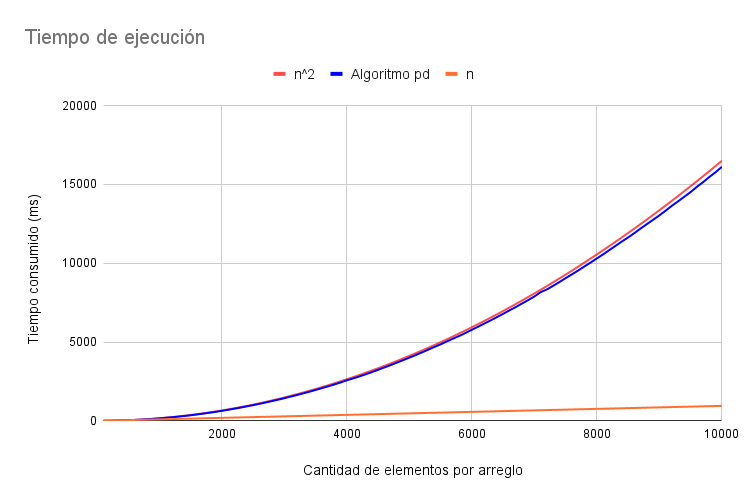
\includegraphics[width=1\textwidth]{img/tiempos_10k_100.png}
    \caption{Medición 1}
\end{figure}

\subsubsection{Análisis de los resultados:}
Con estos resultados es preciso el poder afirmar que el algoritmo PD propuesto, si bien está optimizado para casos particulares, efectivamente tiene una tendencia \textbf{cuadrática} en función del tamaño de los datos de entrada, exactamente como es esperado.
\newpage

\subsection{Segunda medición: Caso particular $x_i$ y $f_i$ constantes}

\subsubsection{Procesamiento y generación de datos de entrada:} 
En este caso se realizaron mediciones en base a crear arreglos de diferentes largos con elementos de valores constantes $C$ y $K$ para $x$ y $f$ respectivamente, yendo de  100 en 100 minutos, cumpliendo $C < K$.

Para obtener un gráfico más legible, los resultados fueron estabilizados usando el promedio de tiempo de 3 por cada prueba.

\begin{figure}[H]
    \centering
    \includegraphics[width=1\textwidth]{img/tiempos_10k_100_xi<f0_constantes.png}
    \caption{Medición 2}
\end{figure}

\subsubsection{Análisis de los resultados:}
Haciendo mediciones con $C < K$ entramos al caso particular $x_i < f_0\forall i $, donde no solo nos encontramos ante una mejora muy significativa en los tiempos del algoritmo, sino además una tendencia \textbf{lineal}. Estos resultados si bien son los esperados debido a la optimización aplicada a nuestro algoritmo, al ser $K$ constante para todo valor de $f$, nos encontramos en un entorno alejado de la realidad, pues los valores de $f$ a recibir serían estrictamente crecientes. 

\newpage

\subsection{Tercera medición: Caso particular $x_i$ y $f_i$ variables}

\subsubsection{Procesamiento y generación de datos de entrada:} 
En este caso, tal como en la \textit{Medición 1}(véase \ref{subsec:medicion1}), se realizaron mediciones en base a crear arreglos para $x$ y $f$ de diferentes largos, yendo de 100 en 100 minutos, con valores pseudoaleatorios para $x$ y pasos pseudoaleatorios para $f$, pero asegurando $x_i < f_0 \forall i $.

Para obtener un gráfico más legible, los resultados fueron estabilizados usando el promedio de tiempo de 3 por cada prueba.

\begin{figure}[H]
    \centering
    \includegraphics[width=1\textwidth]{img/tiempos_10k_100_xi<f0_no_constantes.png}
    \caption{Medición 3}
\end{figure}

\subsubsection{Análisis de los resultados:}
Con estos resultados podemos afirmar que haciendo mediciones con $x_i < f_0 \forall i $ con valores para x y f variables, la optimización efectivamente conlleva a una tendencia \textbf{lineal} y a una significativa mejoría en los tiempos de ejecución de nuestro algoritmo. Cabe aclarar que esta medición refleja el caso en el que nuestra optimización abarca la mayor cantidad de minutos que puede abarcar ($n$) para todas las batallas examinadas pero no es el único caso en el que este se aplique, los minutos pueden variar.
\newpage

\section{Conclusiones}
Hasta este punto hemos logrado observar que la solución de nuestro problema global se compone de subsoluciones que en su determinado minuto fueron las óptimas; inclusive, encontramos la forma en cómo se componen dichas subsoluciones para dar respuesta a problemas más grandes de la misma índole. Dichas caracterisiticas adicionadas a que la problemática nos ofrece un orden natural en el que los hechos se desarrollan o en el que podemos agrandar nuestro problema y que la cantidad de estos mismos sea discreta nos permite plantear una solución mediante programación dinámica. De todas formas, el identificar inicialmente que posiblemente se cumplan estas características en el problema no resta importacia ni complejidad al proceso de entender cómo es que estas caracaterísticas están presentes en el problema ni en cómo se concretizarían teóricamente en la ecuación de recurrencia.



También encontramos relevante el mencionar que, si bien resultó intrincado el identificar y concretizar asertadamente la forma y composición del problema en la ecuación de recurrencia, una vez hecho esto el proceso de la programación propiamente dicha lo consideramos una parte relativamente sencilla, lo que no quita que en este proceso surjan cuestiones importantes a definir, como qué información es imprescindible para resolver correctamente el problema y reconstruir la solucion, que viene estrechamente relacionado con qué datos se deben memorizar, optimizaciones que podamos adaptar y los casos en los que se efectuan estas (como las estudiadas en el desarrollo del presente informe). 
}


\newpage
\end{document}
